For a neural network with $N$ parameters, the Fisher Information is a matrix with $N^2$ entries. To illustrate how large those resulting matrices are, let's consider a network containing 3 hidden layers with a respective width of 128 neurons that gets trained on the $28\times28$ matrices of the MNIST dataset. This network has over $130000$ parameters, which results in over $10^{10}$ entries in the FI. When saving the entries as 32-bit floating point numbers, the matrix would take over 67GB of space. Calculating  this matrix in under 1 hour would require over 2 million entries to be calculated per second. Calculating the full matrix to optimize training is therefore computationally inefficient. That's why we're going to look at an equation for calculating the trace of the Fisher Information, or Fisher Trace for short, through other mathematical objects.\\
Let's first inspect the Fisher Trace by using the chain rule of derivation as
\begin{equation}
	\begin{split}
		\mathrm{tr}(I) &= \sum_{\alpha = 1}^{N_P} I_{\alpha\alpha}\\
		&= \sum_{\alpha = 1}^{N_P} \left\{\underset{(\mathbf{x}_i, \mathbf{y}_i) \in D}{E} \left[\tAbl{}{\theta_\alpha}\ell(f_\theta(\mathbf{x}_i),\mathbf{y}_i)\cdot \tAbl{}{\theta_\alpha}\ell(f_\theta(\mathbf{x}_i),\mathbf{y}_i)\right]\right\}\\
		&= \sum_{\alpha = 1}^{N_P} \left\{ \frac{1}{N} \sum_{i = 1}^{N_D} \left[\sum_{a=1}^{N_O}\left(\pAbl{\ell}{f_\theta(\mathbf{x}_i)_a}\tAbl{f_\theta(\mathbf{x}_i)_a}{\theta_\alpha}\right)\cdot\sum_{b=1}^{N_O}\left(\pAbl{\ell}{f_\theta(\mathbf{x}_i)_b}\tAbl{f_\theta(\mathbf{x}_i)_b}{\theta_\alpha}\right)\right]\right\}\\
		&= \frac{1}{N} \sum_{i = 1}^{N_D} \sum_{a=1}^{N_O} \sum_{b=1}^{N_O} \Bigg[\pAbl{\ell}{f_\theta(\mathbf{x}_i)_a}\pAbl{\ell}{f_\theta(\mathbf{x}_i)_b} \cdot\underbrace{ \sum_{\alpha = 1}^{N_P} \left(\tAbl{f_\theta(\mathbf{x}_i)_a}{\theta_\alpha}\tAbl{f_\theta(\mathbf{x}_i)_b}{\theta_\alpha}\right)}_{\Lambda_{iiab}}\Bigg],
	\end{split} 
\end{equation}
with the amount of parameters $N_P$, the amount of dataset pairs $N_D$ and the output dimension of the network $N_O$. By identifying the entries of the NTK in the last line and simplifying the notation we can rewrite the relation as
\begin{equation}\label{eq:FisherNTKRelation}
	\mathrm{tr}(I) = \underset{(\mathbf{x}_i, \mathbf{y}_i) \in D}{E} \left[\sum_{a,b} \left(\pAbl{\ell}{f_\theta(\mathbf{x}_i)_a}\pAbl{\ell}{f_\theta(\mathbf{x}_i)_b} \cdot \Lambda_{iiab}\right)\right].
\end{equation}
Here it is important to note that there are two main parts on the right hand side: One is the loss derivative with respect to the neural network output, the other consists of diagonal components of the NTK. By diagonal, we refer to components of the NTK where the first to indices refer to the same input point. The loss derivatives are independent of the neural network architecture, whereas the NTK is independent of the loss function.\\
We can also rewrite the Fisher Trace as
\begin{equation}
	\begin{split}
		\mathrm{tr}(I) &= \sum_{\alpha = 1}^{N_P} I_{\alpha\alpha}\\
		&= \sum_{\alpha = 1}^{N_P} \left\{\underset{(\mathbf{x}_i, \mathbf{y}_i) \in D}{E} \left[\tAbl{}{\theta_\alpha}\ell(f_\theta(\mathbf{x}_i),\mathbf{y}_i)\cdot \tAbl{}{\theta_\alpha}\ell(f_\theta(\mathbf{x}_i),\mathbf{y}_i)\right]\right\}\\
		&= \underset{(\mathbf{x}_i, \mathbf{y}_i) \in D}{E} \left\{\sum_{\alpha = 1}^{N_P} \left[\tAbl{}{\theta_\alpha}\ell(f_\theta(\mathbf{x}_i),\mathbf{y}_i)\cdot \tAbl{}{\theta_\alpha}\ell(f_\theta(\mathbf{x}_i),\mathbf{y}_i)\right]\right\}\\
		&= \underset{(\mathbf{x}_i, \mathbf{y}_i) \in D}{E} \left|\nabla_\theta \ell(f_\theta(\mathbf{x}_i),\mathbf{y}_i) \right|^2,
	\end{split}
\end{equation}
which is closely related to the size of the parameter update for Gradient Descent
\begin{equation}
	\theta' - \theta =  \eta \underset{(\mathbf{x}_i, \mathbf{y}_i) \in D}{E} \nabla_\theta \ell(f_\theta(\mathbf{x}_i),\mathbf{y}_i).
\end{equation}
This means that we can split the Fisher Trace, which describes the size of the update of the GD algorithm, into a part depending on the loss function and a part depending on the architecture of the network.\\
Going further we will conduct some experiments to investigate which of those two parts is the dominant driving force in the evolution of the Fisher Trace, and therefore also the driving force behind the training of the neural network. Specifically, we will look at the time evolution of the Fisher Trace in comparison the trace of the NTK to see how similar they evolve during training.

\subsection{Comparison of traces of NTK and Fisher Information}\label{sec:TraceComparisonExperiment}
To test how similar the evolution of the traces of NTK and Fisher Information are, we trained multiple networks on the MNIST dataset explained in \cref{sec:Datasets} and recorded the traces of the FI and NTK. We used networks consisting of 2 hidden layers that were equipped with the ReLU activation function. The network widths varied between $128$ and $784$. The losses used were the $L_p$-Norm loss \cite{LpNormSource}
\begin{equation}
	d_p(f_\theta(\mathbf{x}),\mathbf{y}) = \sqrt[p]{\sum_{i=1}^{N_O} |f_\theta(\mathbf{x}_i) - \mathbf{y}_i|^p},
\end{equation}
the mean-power loss of order $n$
\begin{equation}
	d_n(f_\theta(\mathbf{x}),\mathbf{y}) = \frac{1}{N_O} \sum_{i=1}^{N_O} (f_\theta(\mathbf{x}_i)-\mathbf{y}_i)^n,
\end{equation}
and the softmax-ross-entropy loss \cite{LossExamplePaper}
\begin{equation}
	d(f_\theta(\mathbf{x}),\mathbf{y}) = \sum_{i=1}^{N_O} -\mathbf{y}_i \log(\sigma_i(f_\theta(\mathbf{x}))),
\end{equation}
where we used the definition for distance $d$ from \cref{eq:DistanceLoss}, and a softmax function $\sigma_i$ from \cref{eq:softmax}. The experiment was conducted for orders of $n$ or $p$ equal to $2$, $4$ and $6$. We trained each combination of architecture and loss function for a total of 5 times and calculated mean values and standard deviations of the traces using the results. The networks were trained using the Adam optimizer \cite{adamPaper}.\\
As an illustrative example, the results for $L_2$-norm loss, Mean power loss of order $n=2$, as well as the result for Cross Entropy loss for a network with a width of $128$ neurons are depicted in \cref{fig:MNISTTraceComparison}. The solid line represents the mean of the 5 experiments, the translucent area marks one standard deviation above and under the mean value.\\
\begin{figure}
	\centering
	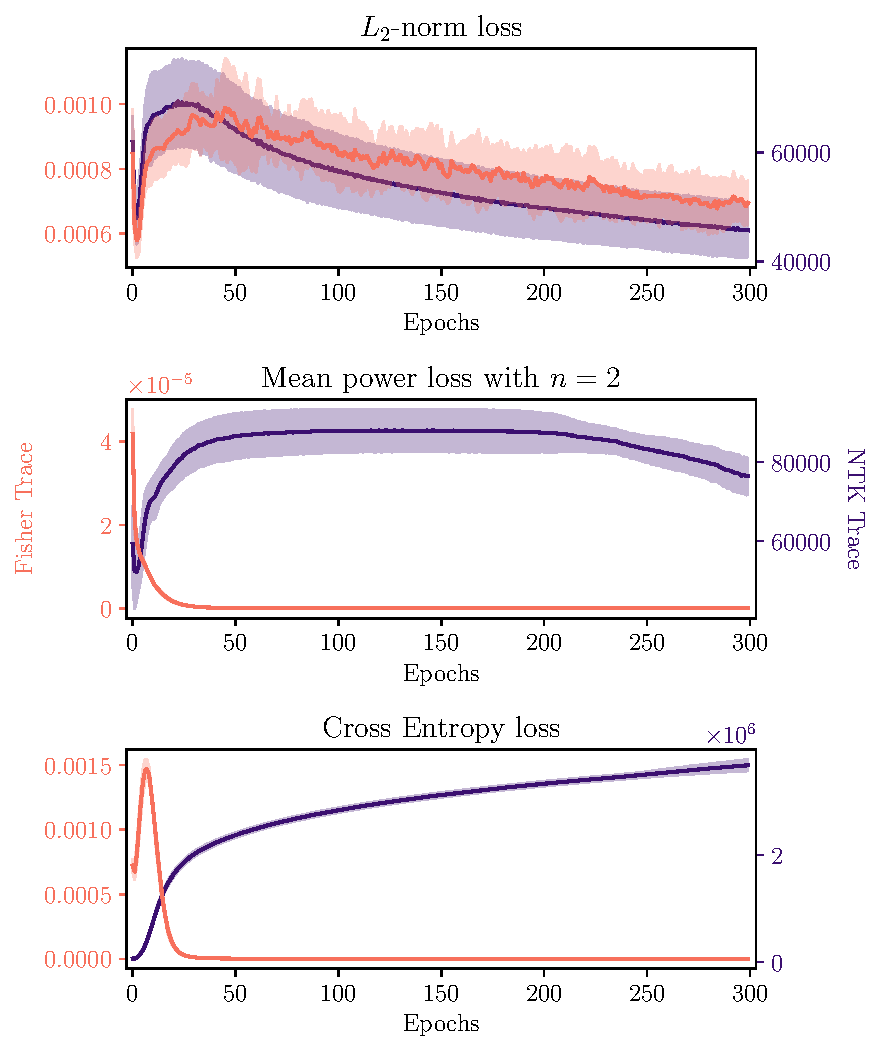
\includegraphics{text/results/FisherNTKComparisonPlots/Triple_comparison_losses2_128.pdf}
	\caption{Trace of NTK and Fisher information during 300 epochs of training on the MNIST dataset using the Adam optimizer. The network consisted of 2 hidden layers with a \emph{width of 128 neurons} that were equipped with the ReLU activation function. The loss functions used for optimization are denoted in each subplot. The solid line represents the mean value of 5 experiments, the translucent area represents one standard deviation from the mean value.}
	\label{fig:MNISTTraceComparison}
\end{figure}
It is visible that for the $L_2$ norm loss of order, the traces evolve almost proportionally to each other, but for the other loss functions they evolve significantly different. This indicates that the loss derivatives in \cref{eq:FisherNTKRelation} play an important role and can't be neglected. The NTK Trace doesn't seem to be a good approximation of the Fisher Trace in general. For which cases the NTK is the driving force of training and can be used as a good approximation for the Fisher Trace needs to be investigated further and can't be answered just from the data generated here.\\
More results from the experiment for different losses and also a larger network width can be found in \cref{sec:TraceExperimentAppendix}. From there it seems like the deviations between the two traces increase for larger network size. 